\newpage
\section{Additional Experiment Results}
\label{sec:additional-results}

\subsection{Predator and Prey}

% \begin{table}[b!]
% %\vspace{-0.4cm} 
% \caption{\small Predator and Prey}
% \centering {\small
%   \begin{tabular}{ccccccc}\specialrule{.1em}{.05em}{.05em} \\[-0.8em]
%     & CON &\begin{tabular}[c]{@{}l@{}}\sched\\ -Top(1)\end{tabular}& \begin{tabular}[c]{@{}l@{}}\sched\\ -Softmax(1)\end{tabular} & DIAL & COMA & IDQN \\ \hline  \\[-0.8em]

%     Average reward    & 2.717  & 2.717   & 4.445    & 11 & 12 &12  \\ \\[-0.8em]
%     Average steps      & 2.717  & 2.717   & 4.445    & 12 & 13 &12 \\\specialrule{.1em}{.05em}{.05em} 
% \end{tabular}
% \label{table:pp}
% }
% \end{table}


\myparagraph{Impact of bandwidth ($L$) and number of schedulable
  agents ($K$)} Due to communication constraints, only $k$ agents can
communicate and scheduled agents can broadcast their message, each of
which has a limited size $l$ due to bandwidth constraints. We see the
impact of $l$ and $k$ on the performance in
Figure~\ref{fig:l_var_add}. As $L$ increases, more information can be
encoded into the message, which can be used by other agents to take
action. Since the encoder and the actor are trained to maximize the
shared goal of all agents, they can achieve higher performance with
increasing $l$. In Figure~\ref{fig:k_var_add}, we compare the cases
where $k=1,2,3$, and FC in which all agents can access the medium,
with $l=1$. As we can expect, the general tendency is that the
performance grows as $k$ increases.


\begin{figure}[t!]
\captionsetup[subfigure]{justification=centering}
  \begin{center}
\hspace{-0.2cm}
    \subfloat[\scriptsize Comm. bandwidth $L$ \newline ($k=1$)]{\label{fig:l_var_add}
      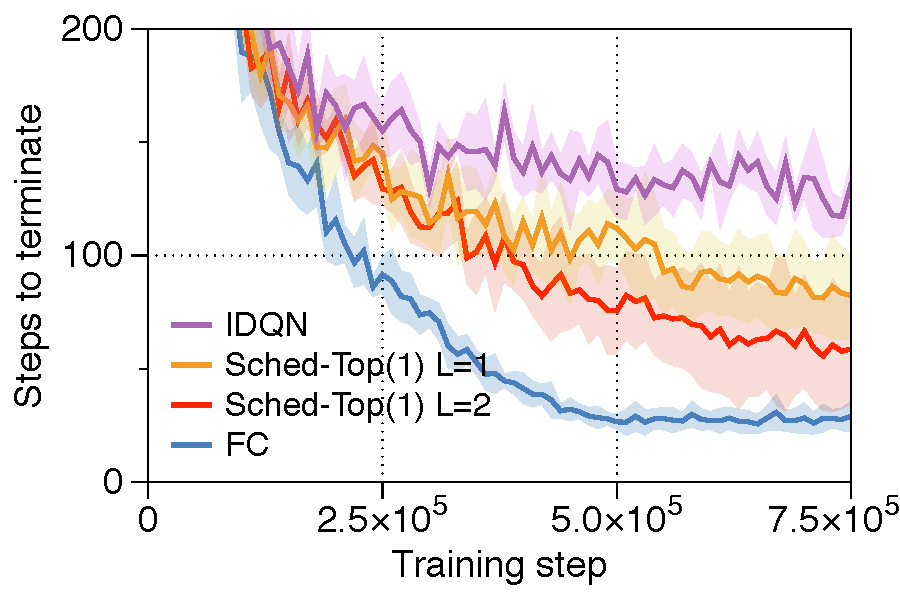
\includegraphics[width=0.3\columnwidth]{add_constraint_l} }
    \subfloat[\scriptsize Sched. constraint $k$ \newline ($l=1$)]
    {\label{fig:k_var_add}
      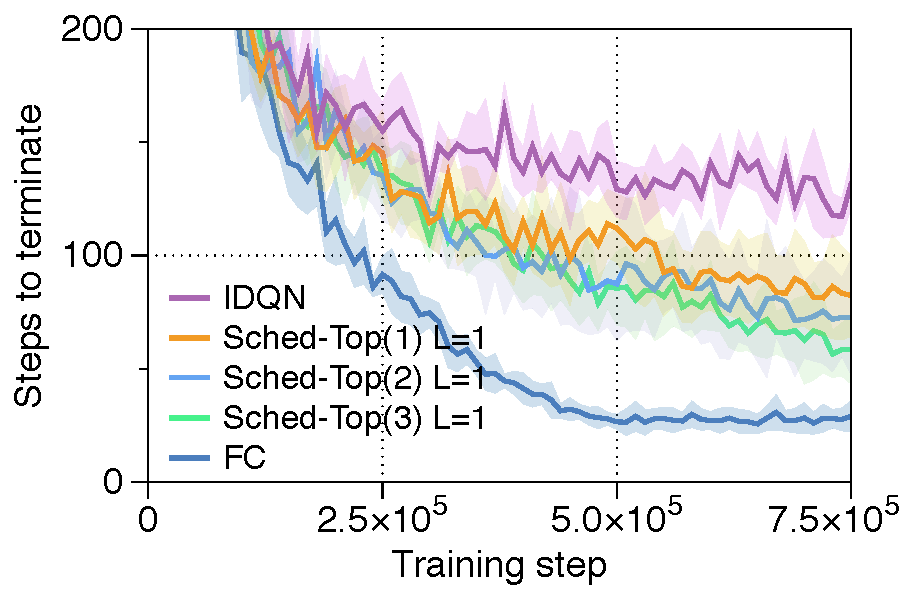
\includegraphics[width=0.3\columnwidth]{add_constraint_k} }
   \subfloat[\scriptsize \sched ~vs. AE  \newline ($k=1$ and $l=1$)] {\label{fig:ae_add}
      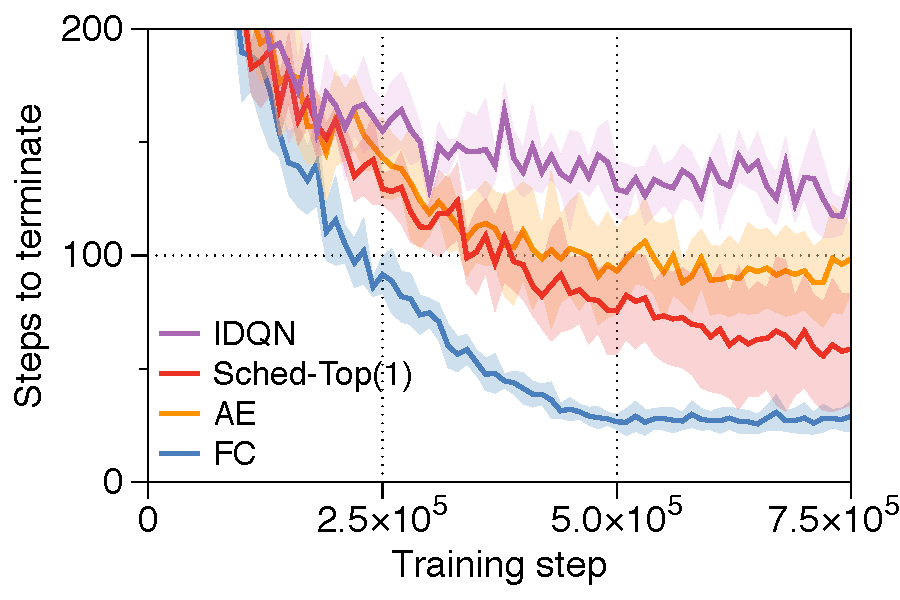
\includegraphics[width=0.3\columnwidth]{add_ae} }
\end{center}
\caption{\small Performance evaluation of \sched. The graphs show the
  average time taken to complete the task, where shorter time is
  better for the agents.}
\label{fig:result_add}
\end{figure}

% \paragraph{Use the history of schedule as an input to the \sched}
% One additional design choice for scheduler is to use previous schedule
% history as an input to the scheduler network.  As shown in
% Figure~\ref{fig:p_pp_add}, using history of schedule improves the
% performance, as well as achieves the stable training.  The intuition
% is that even if one agent observes important information, diverse
% information from others can help to take cooperative actions.

%\begin{wraptable}{R}{0.6\textwidth}
\begin{table}[h!]
%\vspace{-0.4cm} 
\caption{\small Performance with/without encoder}
\centering {\small
  \begin{tabular}{ccc}\hline
    FC & \begin{tabular}[c]{@{}l@{}}\sched\\ -Top(1)\end{tabular}
            & \begin{tabular}[c]{@{}l@{}}Schedule w/\\
                auto-encoder\end{tabular} \\ \hline\hline
    1       & 2.030   & 3.408     \\ \hline 
\end{tabular}
\label{table:ae}
}
\end{table}
%\end{wraptable}


\myparagraph{Impact of joint scheduling and encoding} To study the
effect of jointly coupling scheduling and encoding, we devise a
comparison against a pre-trained auto-encoder \citep{bourlard1988auto,
  hinton1994autoencoders}. An auto-encoder was trained ahead of time,
and the encoder part of this auto-encoder was placed in the Actor's
ENC module in Figure \ref{fig:arch}. The encoder part is not trained
further while training the other parts of network. Henceforth, we name
this modified Actor ``AE''. Figure~\ref{fig:ae_add} shows the learning
curve of AE and other baselines. Table~\ref{table:ae} highlights the
impact of joint scheduling and encoding. The numbers shown are the
performance metric normalized to the FC case in the PP environment.
While \sched -Top(1) took only 2.030 times as long as FC to finish the
PP task, the AE-equipped actor took 3.408 times as long as FC.  This
lets us ascertain that utilizing a pre-trained auto-encoder deprives
the agent of the benefit of joint the scheduler and encoder neural
network in \sched.
% We interpret this superior performance as the isolated
% benefit of jointly training the encoder with the reward signal from
% the environment and the criticism from the centralized critic.


\myparagraph{What messages agents broadcast}

\begin{figure}[h!]
  \centering
    \subfloat[Messages for different relative location of pery.]{\label{fig:msg_o}
  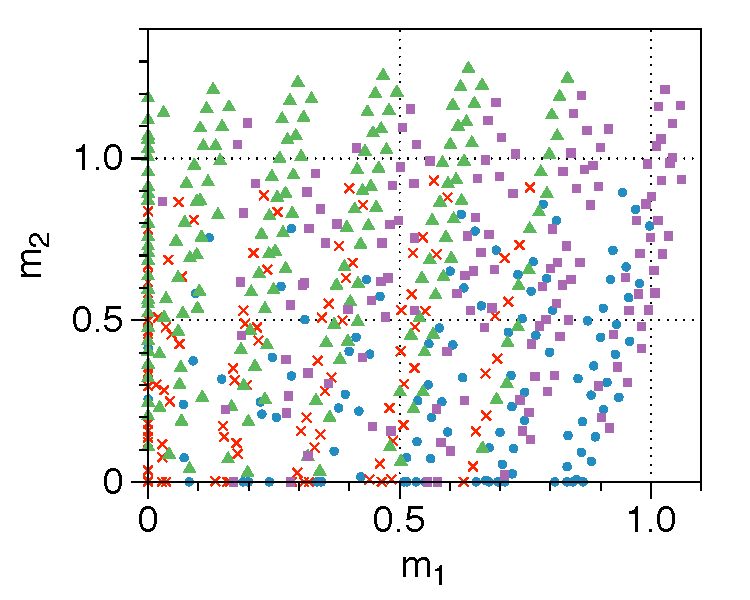
\includegraphics[width=0.4\columnwidth]{4_msgs_o}}
\hspace{0.5cm}
    \subfloat[Messages for different  location of agent.]{\label{fig:msg_a}
  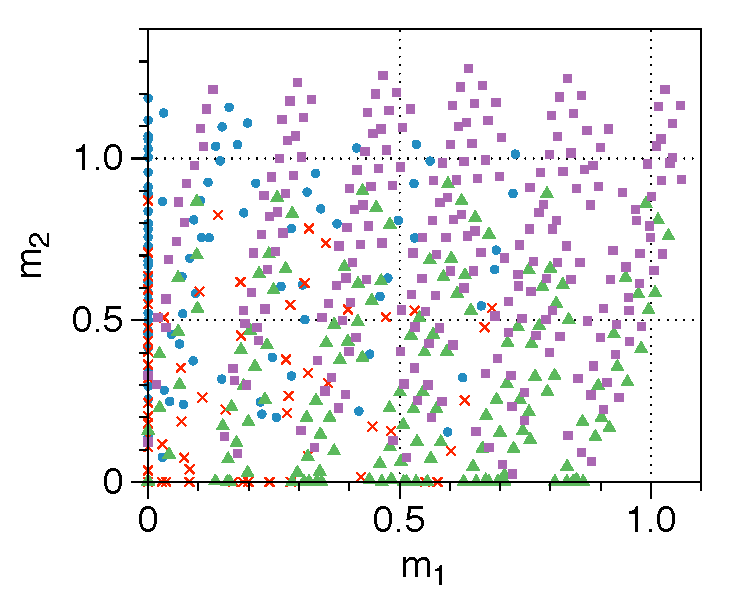
\includegraphics[width=0.4\columnwidth]{4_msgs_a}} 
  \vspace{-0.2cm}
\caption{Projection of encoded messages into 2D plane in PP. }
  \vspace{-0.3cm}
\label{fig:msg_add}
\end{figure}


In Section \ref{sec:pp}, we attempted to understand what the predator
agents communicate when performing PP task where $k=1$ and $l=2$. In
this section, we look into the message in
detail. Figure~\ref{fig:msg_add} shows the projections of the messages
generated by the scheduled agent based on its own observation. In the
PP task, the most important information is the location of the prey,
and this can be estimated from the observation of other agents. Thus,
we are interested in the location information of the prey and other
agents. We classify the message into four classes based on which
quadrant the prey and the predator are included, and mark each class
with different colors. Figure~\ref{fig:msg_o} shows the messages for
different relative location of prey for agents' observation, and
Figure~\ref{fig:msg_a} shows the messages for different locations of
the agent who sends the message. We can observe that there is some
general trend in the message according to the class. We thus conclude
that if the agents observe the prey, they encode into the message the
relevant information that is helpful to estimate the location of the
prey.  The agents who receive this message interpret the message to
select action.

\subsection{Partial Observability Issue in \sched}


In MARL, partial observability issue is one of the major problems, and
there are two typical ways to tackle this issue.  First, using RNN
structure to indirectly remember the history can alleviate the partial
observability issues. Another way is to use the observations of other
agents through communication among them. In this paper, we focused
more on the latter because the goal of this paper is to show the
importance of learning to schedule in a practical communication
environment in which the shared medium contention is inevitable.

  \begin{wrapfigure}{R}{0.39\textwidth}
    \centering
  \vspace{-0.4cm}
  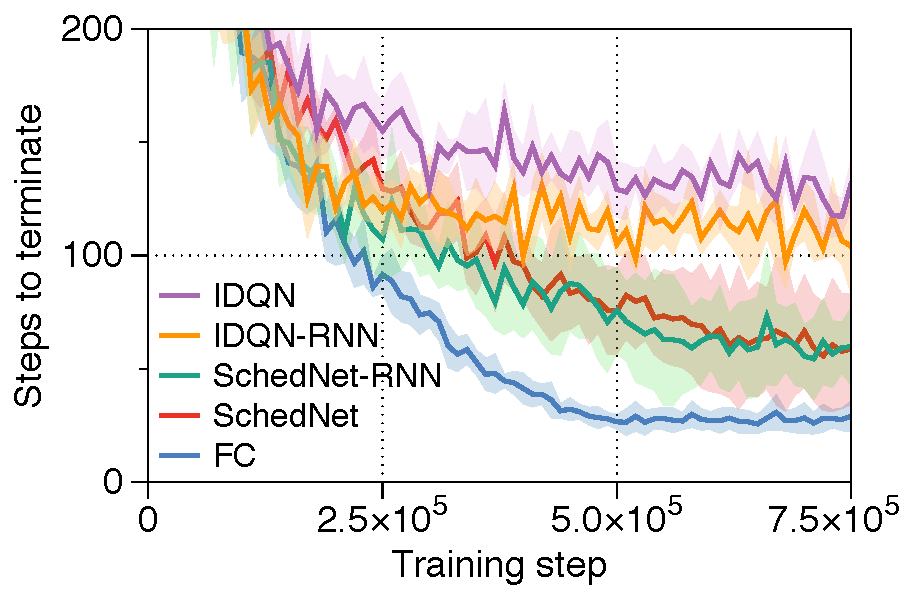
\includegraphics[width=0.36\columnwidth]{rnn}
  \vspace{-0.1cm} \captionof{figure}{\small Impact of applying RNN
    ($k=1$ and $l=2$)}
  \label{fig:rnn}
  \vspace{-0.2cm}
\end{wrapfigure}


Enlarging the observation through communication is somewhat orthogonal
to considering temporal correlation. Thus, we can easily merge
SchedNet with RNN which can be appropriate to some partially
observable environments. We add one GRU layer into each of individual
encoder, action selector, and weight generator of each agent, where
each GRU cell has 64 hidden nodes.

\begin{comment}
  

Figure ~\ref{fig:rnn} shows the result of applying RNN. We implement
IDQN with RNN, and the result shows that the performance of this is
similar to IDQN with feed-forward NN. We also observe that
\sched -RNN and \sched~lie on a comparable performance tier. From
these results, applying RNN does not improve the performance in PP
environment.
%
The main difficulty of this task comes from the fact that it takes a
long time to meet the prey for the first time.  However, RNN is not
really that helpful to meet the prey. It is because the size of the
map is relatively small and the prey move purely randomly without any
pattern so using the history information is not that helpful. We
expect that in a more complex environment, using the recurrent
connection is more helpful.
\end{comment}

Figure ~\ref{fig:rnn} shows the result of applying RNN. We implement
IDQN with RNN, and the results show that the average steps to complete
tasks of IDQN with RNN is slightly smaller than that of IDQN with
feed-forward network. In this case, RNN helps to improve the
performance by tackling the partial observable issue. On the other
hand, SchedNet-RNN and SchedNet achieve similar performance. We think
that the communication in SchedNet somewhat resolves the partial
observable issues, so the impact of considering temporal correlation
with RNN is relatively small. Although applying RNN to SchedNet is not
really that helpful in this simple environment, we expect that in a
more complex environment, using the recurrent connection is more
helpful.

\begin{comment}

There can be two reasons of this. First, the observation range of each
agent is relatively large compared to the size of map. Agent can is
almost covered by the observation range of all agents.


It is observed that agents first find the prey, and then follow it
until all other agents also eventually observe the prey.

The difficult part is to meet the prey for the first time, but RNN
does not help a lot for this.


of the following reasons.
First, the map is relatively small so the agent 


Secondly, the prey move purely randomly without any pattern so
observing the prey in the previous timestep does not help the agent to
acheive the common goal.




Figure ~\ref{fig:rnn} shows the result of applying RNN to \sched. In




SchedNet does not assume any specific neural network
structure as an intrinsic/critical part of its algorithm, where
feed-forward NNs is just one choice. Applying neural networks more
appropriate to the partially observable setting (e.g., RNN) is a
future topic that we will explore.


\end{comment}



\subsection{Cooperative Communication and Navigation}
\label{sec:coop-comm-navig}

  \begin{wrapfigure}{R}{0.39\textwidth}
    \centering
  \vspace{-0.4cm}
  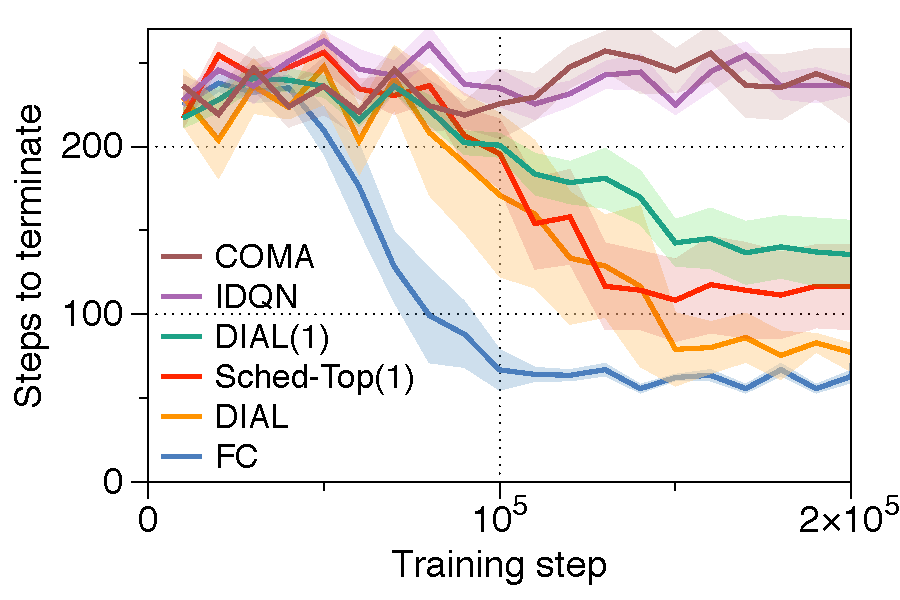
\includegraphics[width=0.36\columnwidth]{a_ccn_baseline}
  \vspace{-0.1cm} \captionof{figure}{\small Comparison with other baselines}
  \label{fig:baseline_ccn}
  \vspace{-0.2cm}
\end{wrapfigure}



\paragraph{Result in CCN} Figure \ref{fig:baseline_ccn} illustrates
the learning curve of 200,000 steps in CCN.  In FC, since all agents
can broadcast their message during execution, they achieve the best
performance. IDQN and COMA in which no communication is allowed, take
a longer time to complete the task compared to other baselines. The
performances of both are similar because no cooperation can be
achieved without the exchange of observations in this environment.  As
expected, \sched~ and DIAL outperform IDQN and COMA.  Although DIAL
works well when there is no contention constraint, under the
contention constraint, the average number of steps to complete the
task in DIAL(1) is larger than that of \sched -Top(1).  This result
shows the same tendency with the result in PP environment.


%%% Local Variables:
%%% mode: latex
%%% TeX-master: "main"
%%% End:
